% Numbers from brand/artifacts/signal_heal_transfer/latency_table.json (v10.1 CUDA microbench).
\paragraph{Transfer inference latency.}
Table~\ref{tab:transfer-latency} reports wall-clock inference on transfer holdout batches
(device=\texttt{cuda}, batch=64, warmup=20, timed=100; includes residual scoring).
N2N uses the wavetable \texttt{n2n\_corrupt\_corrupt} checkpoint zero-shot; domain-trained N2N was not run.
These timings pair with the $R_{\mathrm{blend}}$ transfer board (Table~\ref{tab:transfer-main}).

\begin{table}[t]
  \centering
  \caption{Transfer-domain inference latency (ms/batch; higher is slower). Batch=64; CUDA.}
  \label{tab:transfer-latency}
  \setlength{\tabcolsep}{3.2pt}
  \begin{tabular}{@{}lrrrrrr@{}}
    \toprule
    Method & CWRU & MFPT & MIT-BIH & PTB-XL & CNC & PMU \\
    \midrule
    no-bake & 0.26 & 0.26 & 0.27 & 0.27 & 0.28 & 0.26 \\
    DualCosine & 1.10 & 1.11 & 1.12 & 1.14 & 1.15 & 1.14 \\
    Ours (\texttt{hybrid}) & 3.92 & 6.61 & 2.87 & 1.67 & 1.69 & 1.67 \\
    N2N (WT$\to$dom.) & 0.95 & 0.99 & 0.98 & 0.97 & 0.98 & 0.97 \\
    \bottomrule
  \end{tabular}
\end{table}

\begin{figure}[t]
  \centering
  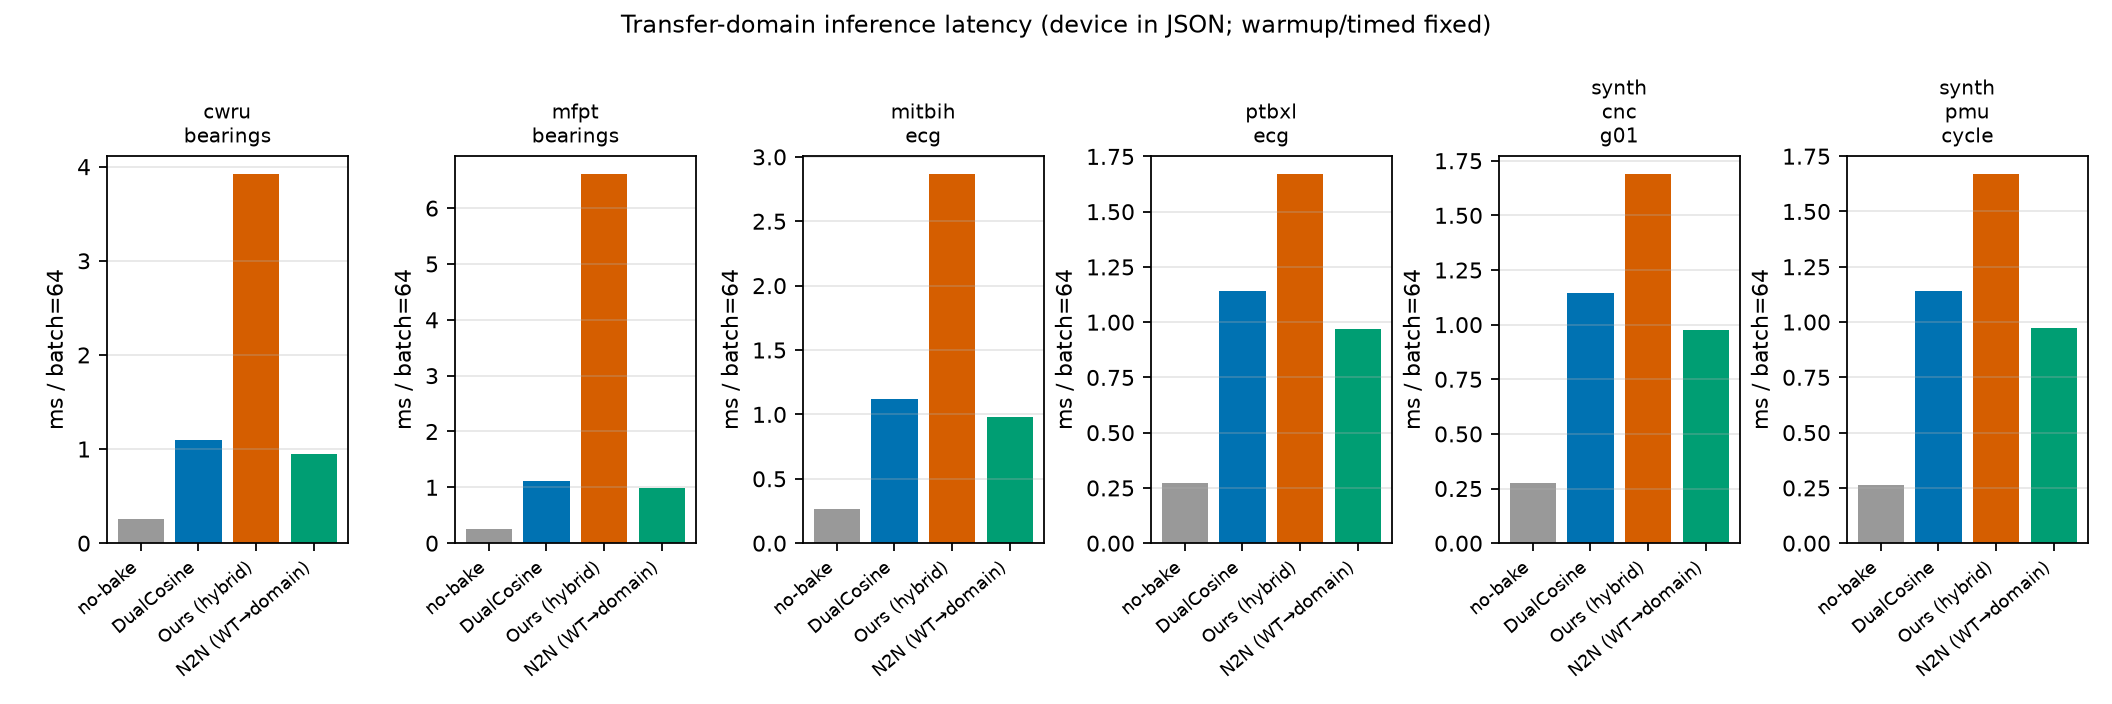
\includegraphics[width=\columnwidth]{figures/fig_signal_heal_transfer_latency.png}
  \caption{Transfer-domain inference latency (ms/batch). N2N is wavetable-trained zero-shot when available.}
  \label{fig:signal-heal-transfer-latency}
\end{figure}
